\begin{frame}
    \frametitle{\problemtitle}
    \begin{itemize}
        \item<+-> \textbf{Problem:} Given $n$ boxes at given positions.
                    Moving a box $d$ positions costs $d^2$. \\
                    What is the minimal cost to make all box positions distinct?
        \item<+-> \textbf{Observation:} The boxes will remain in their original order
                    (they will never overtake each other).
        \item<+-> \textbf{Observation:} Groups of consecutive boxes map to an interval.
        \item<+-> The cost of moving a box from position $p$ to a position $x$,
                    can be modelled with a quadratic function $C_p(x) = (x - p)^2$.
        \begin{itemize}
            \item Example: For one box with original position 3 moved to position $x$, $C_3(x) = (x - 3)^2 = x^2 - 6x + 9$.
        \end{itemize}
        \item<+-> When adding the costs of two groups of boxes that overlap together, \emph{translate} the cost function of the right group of boxes by the size of the left group.
        \begin{itemize}
            \item Example: For two boxes with original position 3, moved such that the left-most box is at position $x$, the summed cost is
                    $C_{3,3}(x) = C_3(x) + C_3(x + 1) = (x - 3)^2 + (x - 2)^2 = 2x^2 - 10x + 13$.
        \end{itemize}
    \end{itemize}
\end{frame}

\begin{frame}[fragile]
    \frametitle{\problemtitle}
    \begin{itemize}
        \item \textbf{Problem:} Given $n$ boxes at given positions.
                Moving a box $d$ positions costs $d^2$. \\
                What is the minimal cost to make all box positions distinct?
        \item The cost of a box at a position $x$, starting at position $p$,
                can be modelled with a quadratic function $C_p(x) = (x - p)^2$.
        \begin{itemize}
            \item For two boxes that start at position 3, the summed cost is
                    $C_{3,3}(x) = C_3(x) + C_3(x + 1) = (x - 3)^2 + (x - 2)^2 = 2x^2 - 10x + 13$.
        \end{itemize}
    \end{itemize}
    \begin{center}Proof by example:\end{center}
    \newcommand\p{3}\newcommand\q{4}\newcommand\C{1}
    \only<2>{\renewcommand\p{1}\renewcommand\q{2}\renewcommand\C{5}}
    \only<3>{\renewcommand\p{0}\renewcommand\q{1}\renewcommand\C{13}}
    \vfill
    \centering
    \begin{tikzpicture}
        \tikzstyle{box}=[draw,thick,fill=black!20,rectangle,minimum size=0.8cm]
        \tikzstyle{arr}=[->,thick]
        \draw (-1, 0) -- (7, 0);
        \foreach \i in {0,1,...,6}{
            \draw (\i, -0.1) -- (\i, 0.1);
            \node[anchor=north] at (\i, -0.1) {\i};
        }
        \node[box,fill=black!10,dotted] at (3, 0.4) {};
        \node[box,fill=black!10,dotted] at (3, 1.2) {};
        \node[box] at (\p, 0.4) {};
        \node[box] at (\q, 0.4) {};
        \only<1>{
            \draw (2.8, 0.9) edge[arr,out=30,in=150] node[above] {0} (\p, 0.9);
            \draw (3.2, 1.2) edge[arr,out=30,in=120] node[above] {1} (\q, 0.8);
        }
        \only<2>{
            \draw (3,   1.2) edge[arr,out=150,in=60] node[above] {4} (\p, 0.8);
            \draw (2.8, 0.8) edge[arr,out=150,in=30] node[above] {1} (\q, 0.8);
        }
        \only<3>{
            \draw (3,   1.2) edge[arr,out=150,in=60] node[above] {9} (\p, 0.8);
            \draw (2.8, 0.8) edge[arr,out=150,in=30] node[above] {4} (\q, 0.8);
        }
    \end{tikzpicture}
    \[ C_{3,3}(\p) = 2 \cdot \p^2 - 10 \cdot \p + 13 = \C \]
\end{frame}

\begin{frame}
    \frametitle{\problemtitle}
    \begin{itemize}
        \item \textbf{Problem:} Given $n$ boxes at given positions.
                Moving a box $d$ positions costs $d^2$. \\
                What is the minimal cost to make all box positions distinct?
        \item<+-> \textbf{Solution:} Add every box from left to right, maintaining the optimal placement
                    by maintaining the cost function for every group of boxes.
        \item<+-> If two groups of boxes touch or overlap, merge them into one group
                    by summing their (possibly translated) costs.
        \begin{itemize}
            \item This new group may overlap with its preceding group after the merge, so merge recursively.
        \end{itemize}
        \item<+-> For every group with cost $C(x) = ax^2 + bx + c$, the minimal cost is:
        \[ C\left(\left\lfloor \frac{-b}{2a} + \frac12\right\rfloor \right) \]

        \item<+-> The total runtime is $\mathcal O(n)$ (after sorting): we do at most $n - 1$ merges.
    \end{itemize}
    \solvestats
\end{frame}
